%%=============================================================================
%% Inleiding
%%=============================================================================

\chapter{\IfLanguageName{dutch}{Inleiding}{Introduction}}%
\label{ch:inleiding}


De artikel van \textcite{StatistiekVlaanderen2023} biedt een gedetailleerde analyse van de Vlaamse leeftijdspiramide, die een vergrijzende bevolking toont met een brede bovenkant en een smalle basis. Deze bron bespreekt de significante aanwezigheid van de babyboomgeneratie binnen de huidige demografie en de stijgende proportie oudere volwassenen in de bevolking, in het bijzonder in kustgemeenten waar meer dan een derde van de bevolking ouder is dan 65 jaar. Daarnaast benadrukt het de krimpende jongere demografie, wat wijst op een dalend geboortecijfer. 
\\
Deze demografische schuiving brengt aanzienlijke uitdagingen met zich mee. Het vereist een herbeoordeling van de beschikbare middelen en een strategische benadering om de levenskwaliteit en zorg van de senioren te waarborgen. Dit onderstreept het fundamentele belang van onderzoek dat zich focust op het optimaliseren van de levenskwaliteit en de ondersteunende diensten voor onze senioren.
\begin{figure}[h]
    \centering
    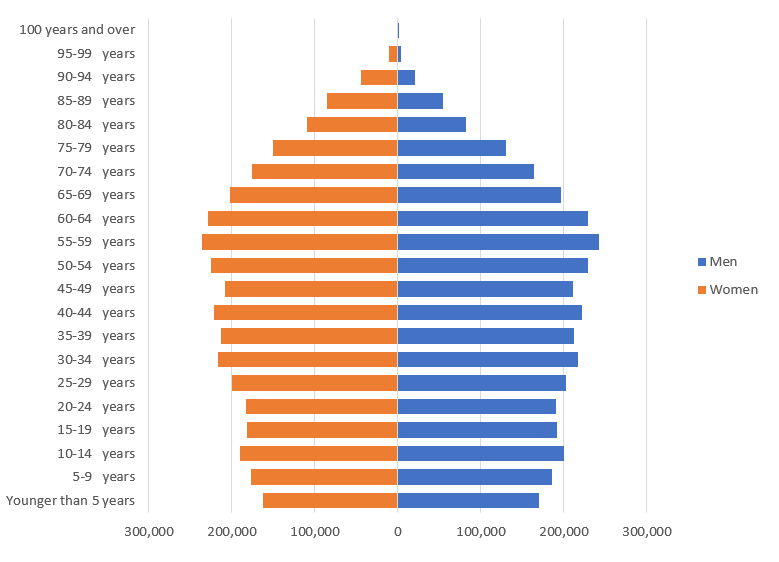
\includegraphics[width=0.8\textwidth]{graph_statistiekVlaanderen.png}
    \captionsetup{justification=centering}
    \caption{Het uitvoeringsplan voor de evaluatieprocedure.}
    \label{fig:plan_methodologie}
\end{figure}
\FloatBarrier

Deze doelstelling zal worden bereikt door een grondige evaluatie van diverse transcripties dit door ASR models gegenereerd worden, met als doel het selecteren van de meest accurate transcriptie.
\section{\IfLanguageName{dutch}{Probleemstelling}{Problem Statement}}%
\label{sec:probleemstelling}
Deze bachelorproef confronteert de uitdaging van misverstanden en miscommunicatie die voortvloeien uit het gebruik van 'Secondary Babytalk' in de interacties tussen zorgverleners en oudere patiënten. Het onderzoeksprobleem richt zich op het identificeren van het meest effectieve speech-to-text model dat deze unieke vorm van communicatie kan decoderen. De noodzaak om een duidelijk, respectvol en verstaanbaar communicatiekader te waarborgen binnen de zorgsector, vormt de kern van deze probleemstelling. Daarbij is het essentieel dat het geselecteerde model accuraatheid combineert met sensitiviteit voor de nuances in taalgebruik bij oudere patiënten.
Het belang van dit onderzoek komt tot uiting in de meerwaarde die het zal bieden voor oudere patiënten en studenten verpleegkunde. Door een verfijnde speech-to-text technologie te identificeren die 'Secondary Babytalk' nauwkeurig kan transcriberen, streven we naar het verbeteren van de communicatie in de zorgsector. Dit is niet alleen van cruciaal belang voor de waardigheid en het welzijn van ouderen, maar ook voor het onderwijs en de professionele ontwikkeling van toekomstige verpleegkundigen.



\section{\IfLanguageName{dutch}{Onderzoeksvraag}{Research question}}%
\label{sec:onderzoeksvraag}

De centrale onderzoeksvraag van deze bachelorproef zal als volgt zijn:\\


\say{Hoe kunnen we spraak-naar-tekstmodellen evalueren om te bepalen welk model optimaal presteert voor de specifieke usecase van spraaktranscriptie?}\\
\break
Het beantwoorden van deze vraag is fundamenteel voor het verbeteren van de communicatie tussen zorgverleners en oudere patiënten. Om een grondiger en omvattend antwoord op deze vraag te formuleren, worden de volgende deelvragen onderzocht:

\begin{itemize}
    \item Wat houd een speech-to-text model in precies en waar bevindt het zich in de wereld van kunstmatige intelligentie?
    \item Welke modellen zijn beschikbaar op de markt om te testen?
    \item Wat zijn relevante criteria om dergelijke modellen te evalueren?
\end{itemize}
\section{\IfLanguageName{dutch}{Onderzoeksdoelstelling}{Research objective}}%
\label{sec:onderzoeksdoelstelling}

De hoofddoelstelling van deze bachelorproef is het selecteren van het meest accurate spraak-naar-tekstmodel dat beschikbaar is op de markt, om vervolgens gebruikt te worden in verdere studies gericht op de communicatie tussen zorgverleners en oudere patiënten. 



Het succes van dit onderzoek zal concreet gemeten worden door de volgende: 

\begin{itemize}
    \item Een verzameling van divers opnames van accenten in België vrij van bias. daarna het inzetten van een open-source evaluatiebibliotheek om de prestaties van diverse modellen objectief te kunnen vergelijken. 
    \item Een duidelijk en concreet evaluatieresultaat verkrijgen, dat als solide basis dient voor de selectie van het meest nauwkeurige model:you
    

\end{itemize}

Verder streven we naar het ontwikkelen van een proof-of-concept applicatie die de functionaliteiten van een 'Elderspeak' monitoringapplicatie voor studenten verpleegkunde vergemakelijkt.

\section{\IfLanguageName{dutch}{Opzet van deze bachelorproef}{Structure of this bachelor thesis}}%
\label{sec:opzet-bachelorproef}


De rest van deze bachelorproef is als volgt opgebouwd:

In Hoofdstuk~\ref{ch:stand-van-zaken} wordt een overzicht gegeven van de stand van zaken binnen het onderzoeksdomein, op basis van een literatuurstudie.

In Hoofdstuk~\ref{ch:methodologie} wordt de methodologie toegelicht en worden de gebruikte onderzoekstechnieken besproken om een antwoord te kunnen formuleren op de onderzoeksvragen.

In Hoofdstuk~\ref{ch:onderzoek} wordt het onderzoek uitgevoerd, waarbij alle resultaten van de transcripties en evaluaties worden gepresenteerd. Op basis van deze gegevens wordt vervolgens een onderbouwde conclusie getrokken.

In Hoofdstuk~\ref{ch:poc} De focus zal liggen op het demonstreren van de ontwikkelde mobiele applicatie.

In Hoofdstuk~\ref{ch:conclusie}, tenslotte, wordt de conclusie gegeven en een antwoord geformuleerd op de onderzoeksvragen. Daarbij wordt ook een aanzet gegeven voor toekomstig onderzoek binnen dit domein.